\documentclass[12pt, fleqn]{article}
\usepackage{amsmath}
\usepackage{geometry, titling, enumitem, graphicx, float, listings, xcolor}

\graphicspath{{./images/}}

\geometry{
    paper=a4paper,
    top=64pt,
    bottom=64pt
}

\definecolor{bg}{rgb}{0.96,0.96,0.96}
\definecolor{codegray}{rgb}{0.5,0.5,0.5}
\definecolor{codepurple}{rgb}{0.58,0,0.82}
\definecolor{backcolour}{rgb}{0.95,0.95,0.92}

\lstset{
    basicstyle=\ttfamily\small,
    backgroundcolor=\color{gray!5},
    frame=single,
    rulecolor=\color{gray!20},
    framesep=16pt,
    xleftmargin=16pt,
    xrightmargin=16pt,
    captionpos=b
}

\renewcommand{\arraystretch}{1.2}
\setlength{\tabcolsep}{8pt}

\NewDocumentCommand{\course}{m}{\gdef\thecourse{#1}}
\NewDocumentCommand{\authors}{m}{\gdef\theauthors{#1}}
\NewDocumentCommand{\professor}{m}{\gdef\theprofessor{#1}}
\NewDocumentCommand{\semester}{m}{\gdef\thesemester{#1}}

\renewcommand{\maketitle}{
    \begin{titlepage}
        \begin{center}
            {\scshape Universidade Federal do Rio Grande do Sul\\Instituto de Informática} \\
            \vspace*{\fill}
            {\large \thecourse} \\[16pt]
            {\Huge \thetitle} \\[36pt]
            \theauthors \\
            \vspace*{\fill}
            \theprofessor \\[2pt]
            \thesemester
        \end{center}
    \end{titlepage}
}

\course{Circuitos Digitais – INF01058}
\title{LAB 06 – Display de 7 segmentos}
\authors{
    Ana Cláudia Rodrigues — 343123 \\[2pt]
    Bruno Samuel Ardenghi Gonçalves — 550452
}
\professor{Prof. Sérgio Bampi}
\semester{2025/1}

\begin{document}

\maketitle

\section{Introdução}

Neste laboratório desenvolvemos um decodificador de binário para a representação hexadecimal em um display de 7 segmentos. Para verificação do projeto, foi utilizada a saída da ULA (com operação artmética de soma e operações lógicas de AND, OR e NOT) elaborada previamente (laboratório 5). O projeto foi implementado e simulado pelo software Quartus, posteriormente sintetizado e testado em uma FPGA Cyclone III D0 (modelo EP3C16F484C6).

\subsection{Entradas}

\begin{itemize}
    \item $S_{3-0}$: "código" de entrada de 4 bits (saída da ULA, entrada do decodificador)
\end{itemize}

\subsection{Saídas}

\begin{itemize}
    \item $S_{A-G}$: segmentos do display (onde o resultado será exibido)
\end{itemize}

\subsection{Módulos e funções}

\begin{itemize}
    \item Decodificador 4:16
    \newline
        OBS: decodificação feita de modo a gerar correspondência binário-hexadecimal
    \item Função ISOP (ou IPOS) para implementação das saídas do display
    \begin{itemize}
        \item $S_{A}=\overline{A}\overline{B}\overline{C}D+A\overline{B}CD+AB\overline{C}D+\overline{A}B\overline{C}\overline{D}$
        \item $S_{B}=\overline{A}B\overline{C}D+BC\overline{D}+AB\overline{D}+ACD$
        \item $S_{C}=ABC+\overline{A}\overline{B}C\overline{D}+AB\overline{D}$
        \item $S_{D}=\overline{A}\overline{B}\overline{C}D+\overline{A}B\overline{C}\overline{D}+A\overline{B}C\overline{D}+BCD$
        \item $S_{E}=\overline{B}\overline{C}D+\overline{A}D+\overline{A}B\overline{C}$
        \item $S_{F}=AB\overline{C}D+\overline{A}CD+\overline{A}\overline{B}D+\overline{A}\overline{B}C$
        \item $S_{G}=AB\overline{C}\overline{D}+\overline{A}\overline{B}\overline{C}+\overline{A}BCD$
    \end{itemize}
\end{itemize}

\section{Resultados}

\begin{table}[H]
    \centering
    \begin{tabular}{|l | c|}
        \hline
        \textbf{Total de elementos lógicos} & 18 \\
        \hline
        \textbf{Total de pinos} & 19 \\
        \hline
        \textbf{Área total} & 37 \\
        \hline
    \end{tabular}
    \caption{Consumo de recursos do FPGA em área}
\end{table}

\begin{table}[H]
    \centering
    \begin{tabular}{|l | c|}
        \hline
        \textbf{Frequencia máxima} & 129.8 MHz \\
        \hline
        \textbf{Atraso crítico} & 7.204 ($A_1 \to S_G$) \\
        \hline
    \end{tabular}
    \caption{Frequência máxima de operação e atraso crítico (Slow, 85°C)}
\end{table}

\section{Capturas de tela}

\begin{figure}[H]
    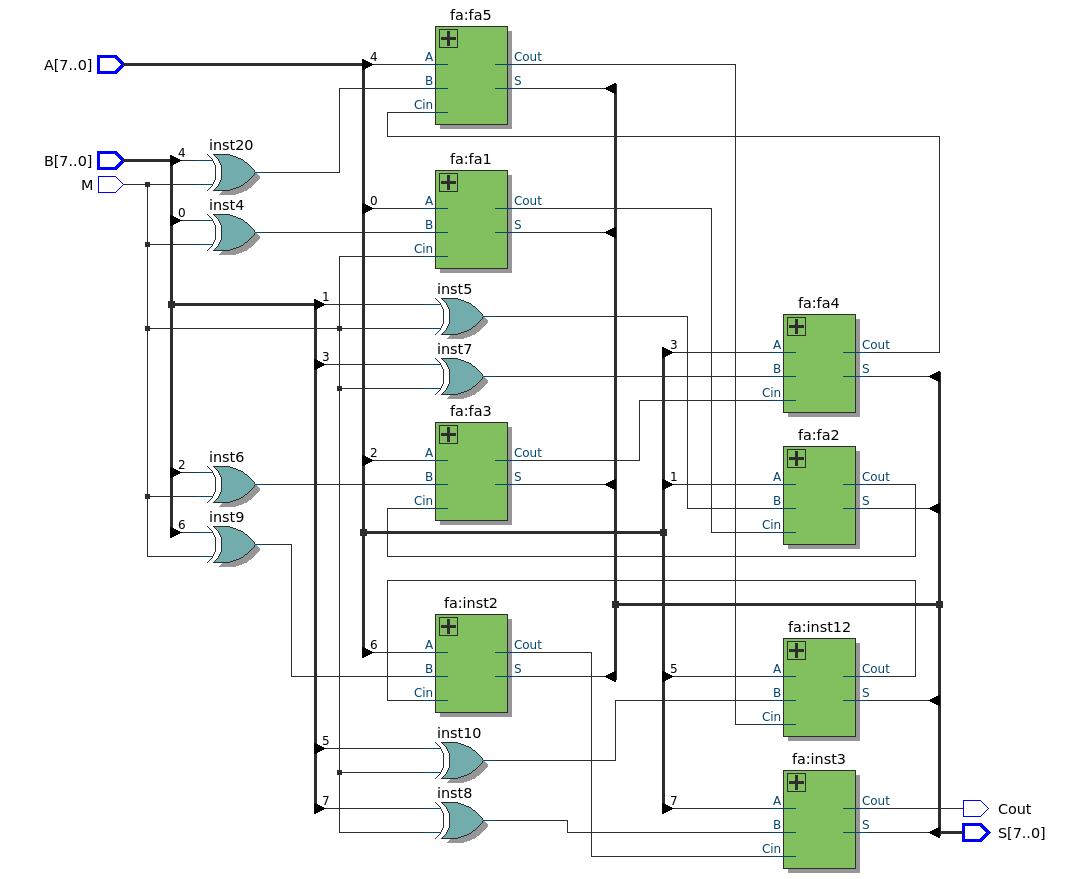
\includegraphics[width=\textwidth]{netlist.png}
    \caption{Captura de tela do netlist}
\end{figure}

\begin{figure}[H]
    
    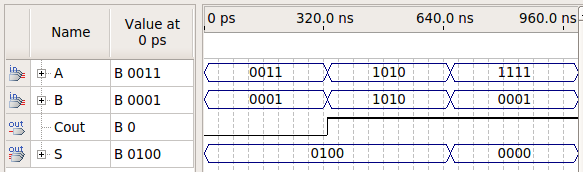
\includegraphics[width=\textwidth]{waveform.png}
    \caption{Captura de tela da simulação em forma de onda com atraso}
\end{figure}

\section{Arquivo de restrições}

\begin{lstlisting}[caption=constraints.sdc]
create_clock -name clk -period 10
set_clock_uncertainty -from clk 0.1

set_input_delay -clock clk -max 0.2 [all_inputs]
set_input_delay -clock clk -min 0.01 [all_inputs]
set_output_delay -clock clk -max 0.2 [all_outputs]
set_output_delay -clock clk -min 0.01 [all_outputs]    
\end{lstlisting}

\end{document}
